%!Mode:: "TeX:UTF-8"
\documentclass{beamer}
\usepackage{xeCJK}
\usepackage{xcolor}
\usepackage{listings}
\usepackage{soul}
%\usepackage{ulem}

%\setCJKmainfont{AR PL SungtiL GB}
\setCJKmainfont{SimSun}

\definecolor{dkgreen}{rgb}{0,0.6,0}
\definecolor{gray}{rgb}{0.5,0.5,0.5}
\definecolor{mauve}{rgb}{0.58,0,0.82}

\lstset{
    language=sh,
    %basicstyle=\footnotesize\ttfamily,
    basicstyle=\scriptsize\ttfamily,
    frameround=tttt,
    frame=single,
    keywordstyle=\color{blue},
    commentstyle=\color{dkgreen},
    stringstyle=\color{mauve},
    numbers=left,
    numberstyle=\tiny\color{gray},
    numbersep=5pt,
    escapeinside={(*@}{@*)},
    %otherkeywords={$, \{, \}, \[, \]},
}

\setbeamertemplate{navigation symbols}{}
\usetheme{Madrid}
\begin{document}

\title{Git + CMT + Dyb2Sim}
\author{
    \texorpdfstring{林韬
                    \newline
                    \href{mailto:lintao@ihep.ac.cn}
                    {\footnotesize\ttfamily{lintao@ihep.ac.cn}}}
                    {Lin Tao}
}

\institute{IHEP}

\maketitle

\begin{frame}
    \frametitle{OUTLINE}
    \tableofcontents
\end{frame}

\section{git简介}
    %!Mode:: "TeX:UTF-8"
%\begin{frame}
%    \frametitle{OUTLINE}
%    \begin{itemize}    
%        \item
%    \end{itemize}
%\end{frame}

\begin{frame}
    \begin{center}
        \LARGE \tt{GIT}
    \end{center}
\end{frame}

\begin{frame}
    \frametitle{Git基础}
    \begin{itemize}    
        \item 版本控制的概念
            \begin{description}
                \item[版本控制\footnote{\url{http://zh.wikipedia.org/wiki/\%E7\%89\%88\%E6\%9C\%AC\%E6\%8E\%A7\%E5\%88\%B6}}] 
                    是维护工程蓝图的标准作法,
                    能追踪工程蓝图从诞生一直到定案的过程。
                    此外,版本控制也是一种软件工程技巧,
                    借此能在软件开发的过程中,
                    确保由不同人所编辑的同一程式档案都得到同步。
            \end{description}
        \item 关于GIT
            \begin{description}
                \item[Git\footnote{\url{http://zh.wikipedia.org/wiki/Git}}] 
                    是一个由Linus Torvalds
                    为了更好地管理linux内核开发
                    而创立的{\em 分布式}版本控制/软件配置管理软件。
            \end{description}
        \item 一个重要概念\footnote{\url{http://git-scm.com/book/en/Getting-Started-Git-Basics}}
            \begin{itemize}
                \item Git关心文件数据的整体是否发生变化。
                \item 其他版本管理系统则关心具体内容的差异。
            \end{itemize}
    \end{itemize}
\end{frame}

\begin{frame}
    \frametitle{git的版本控制模型}
    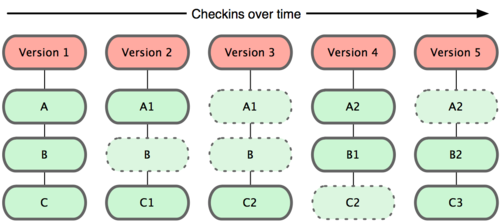
\includegraphics[width=10cm,keepaspectratio]{data/GitRevisionModel.png}

    每个版本都是对这个项目的快照(snapshot)。
\end{frame}

\begin{frame}
    \frametitle{其他系统的版本控制模型}
    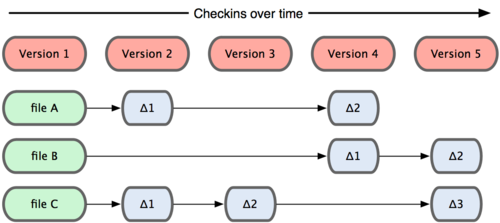
\includegraphics[width=10cm,keepaspectratio]{data/OtherRevisionModel.png}
\end{frame}

\begin{frame}
    \frametitle{分布式工作流程\footnote{\url{http://git-scm.com/book/en/Distributed-Git-Distributed-Workflows}}}
    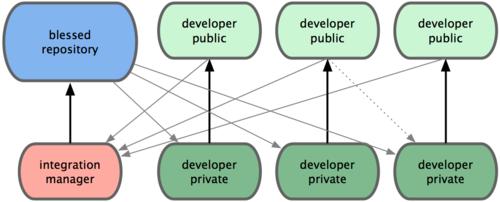
\includegraphics[width=10cm,keepaspectratio]{data/GitDistributedWorkflow.png}
    \begin{block}{我们的开发模式}
        \begin{itemize}
            \item 公共的仓库,由管理员负责
            \item 个人的仓库,由开发者自己管理
            \item 如果要将个人的代码合并如公共的仓库,
                  提交Pull Request,告诉管理员仓库的url和分支名。
        \end{itemize}
    \end{block}
\end{frame}

\begin{frame}
    \frametitle{Git的数据流}
    \begin{columns}
        \column{6.0cm}
            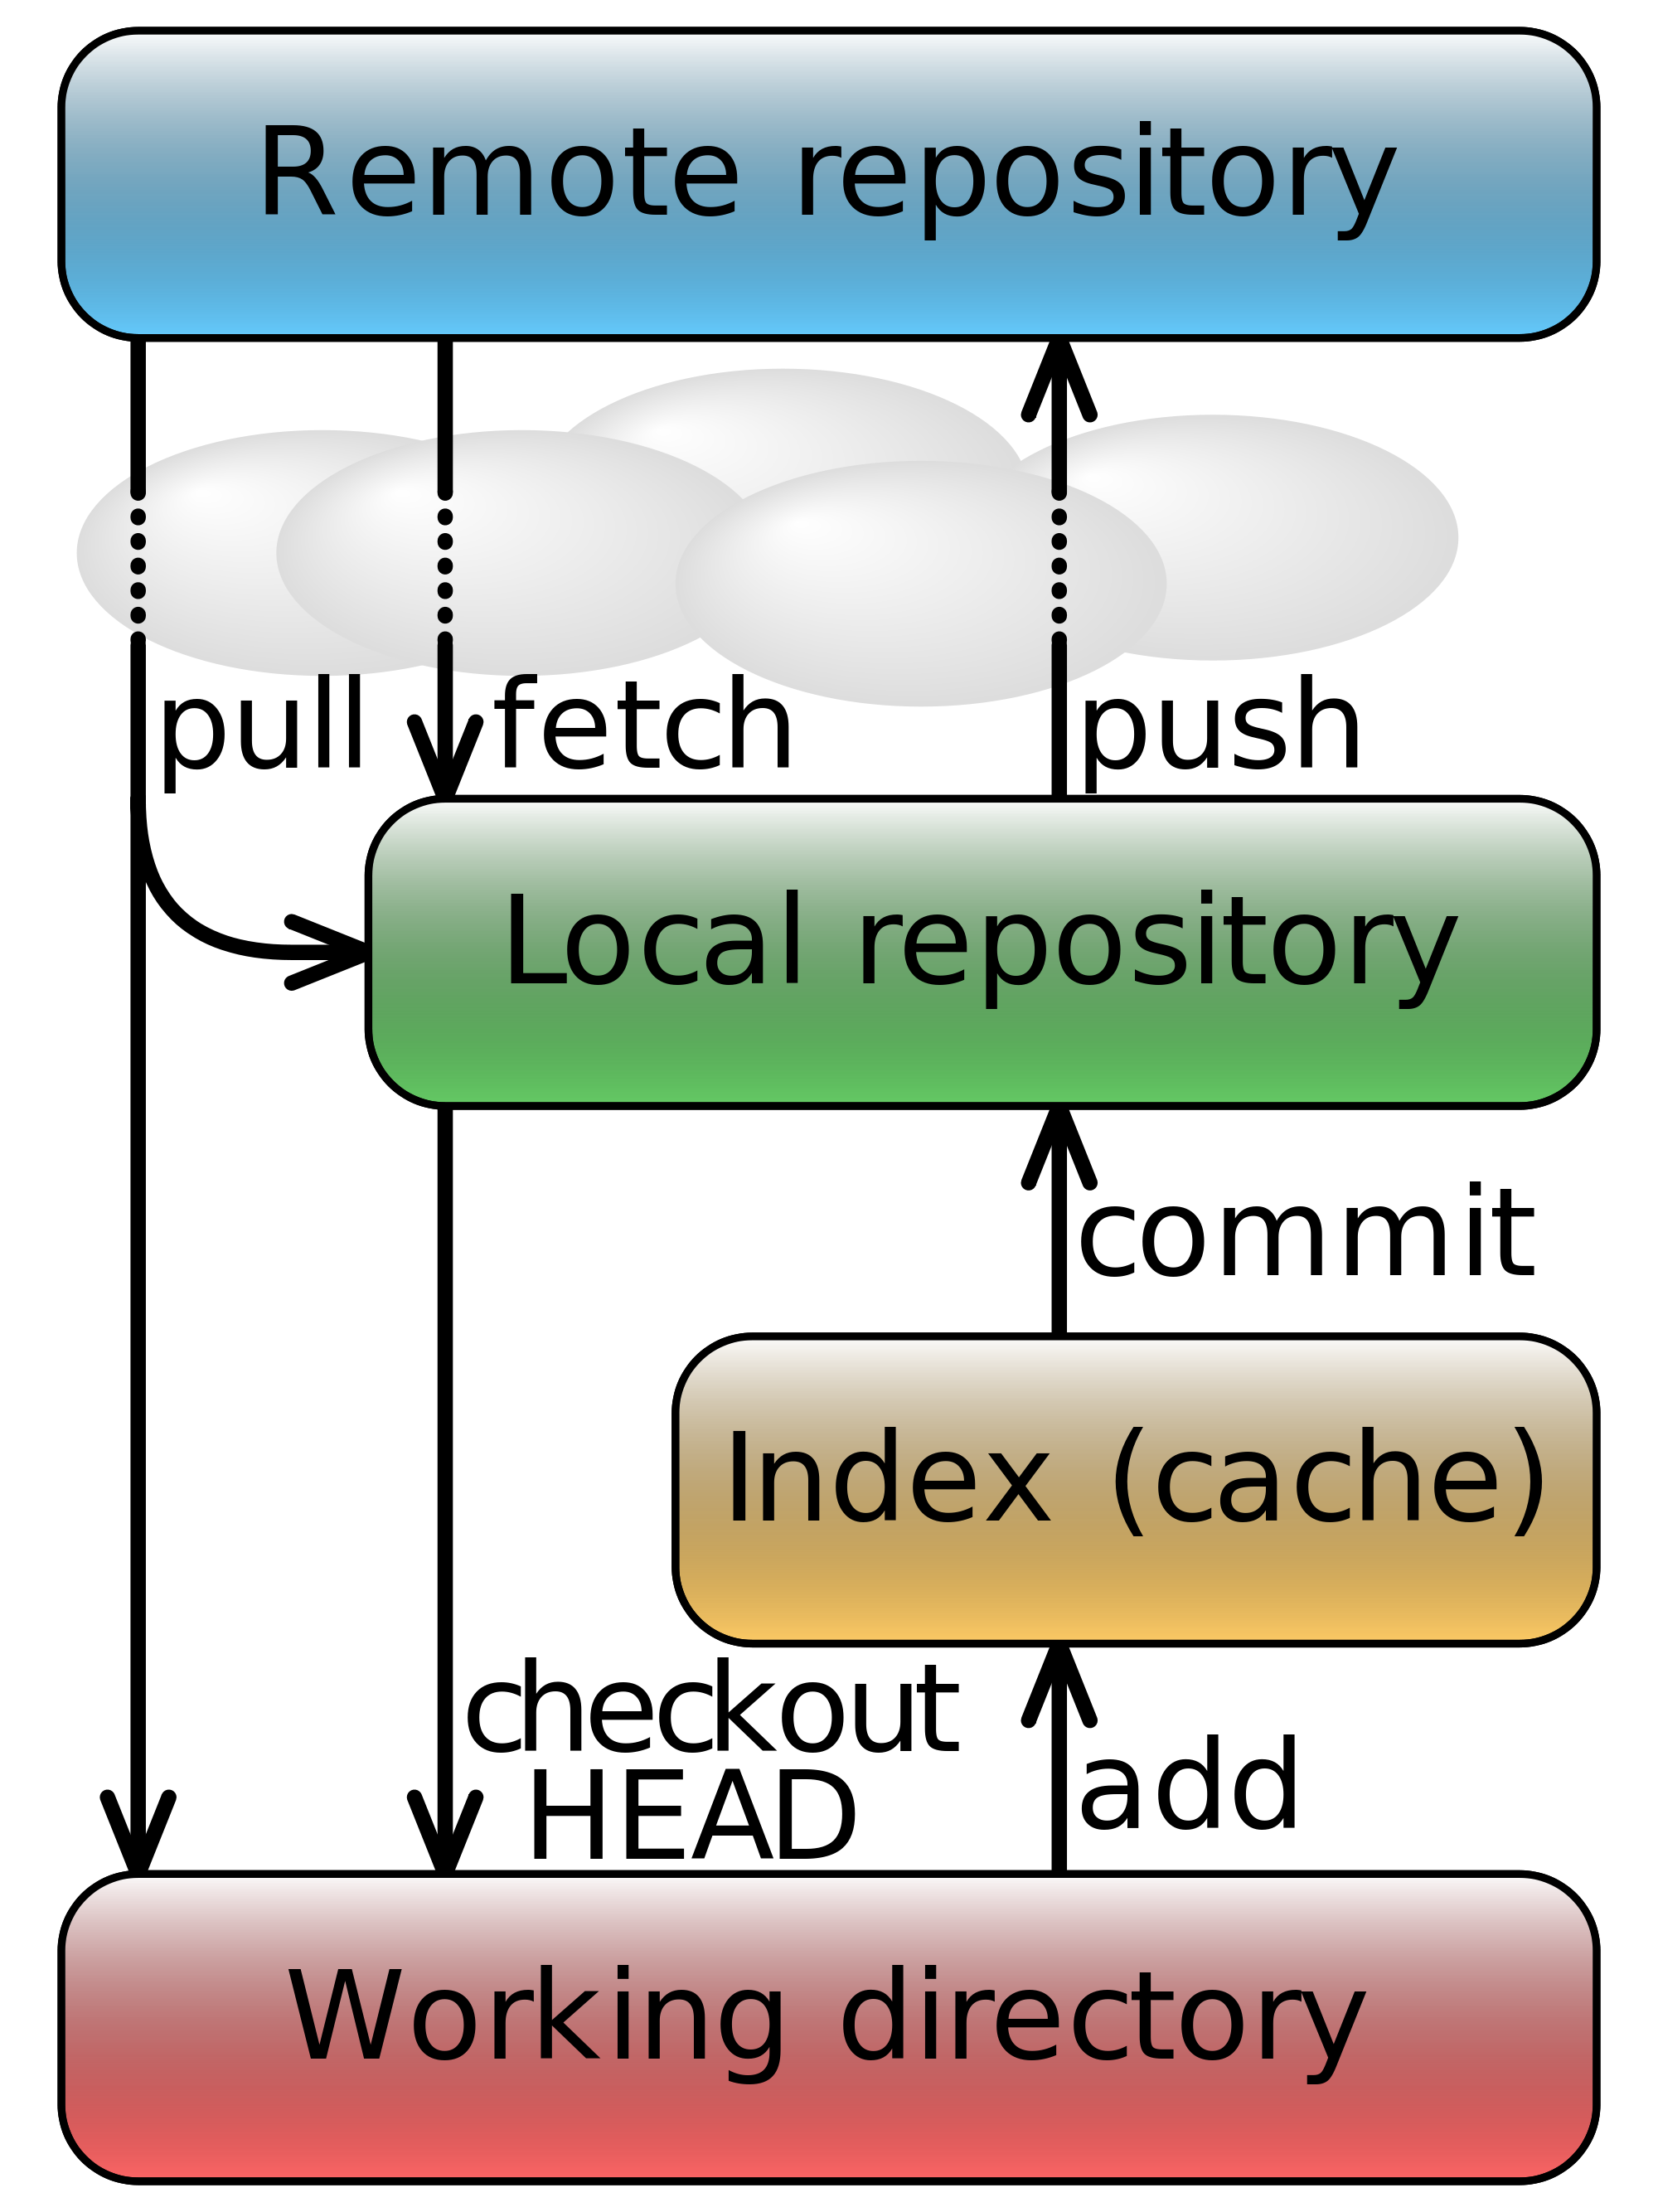
\includegraphics[height=8cm,keepaspectratio]{data/GitDataFlowSimplified.png}
            \label{pic:DataFlow}
        \column{4.5cm}
            \begin{itemize}
                \item 远程仓库
                \item 本地仓库
                \item 工作目录
            \end{itemize}
    \end{columns}
\end{frame}

\begin{frame}
    \frametitle{Git与CVS的部分区别
        \footnote{\scriptsize \url{http://stackoverflow.com/questions/802573/difference-between-git-and-cvs}}}
    \begin{block}{Git}
        \begin{itemize}
            \item 分布式仓库。用户无需任何服务器,在本地即可进行所有操作。
            \item 原子操作。操作要么完全成功,要么完全失败。
            \item 改动是对于整个项目。因此很容易回退到特定版本。
            \item 版本号也是基于整个项目。一个版本对应一个快照。
            \item 分支功能强大。包括创建合并等。
        \end{itemize}
    \end{block}
    \begin{block}{CVS}
        \begin{itemize}
            \item 集中式仓库。需要设置仓库的服务器,合并等操作都由服务器完成。
            \item 非原子操作。如果某个操作在中间被打断,可能处于不一致的状态。
            \item 改动是对于一个文件而言。我们可以checkout一些特定的文件。
            \item 版本号是对于文件而言。我们需要建立tag关联各个文件,
                  以指向特定的状态。
        \end{itemize}
    \end{block}
\end{frame}

\begin{frame}
    \frametitle{Git与SVN的部分区别
        \footnote{\scriptsize \url{http://stackoverflow.com/questions/871/why-is-git-better-than-subversion}}}
        \begin{quote}
            Git is not better than Subversion. But is also not worse. It's
            different.
        \end{quote}

        \begin{quote}
            The key difference is that it is decentralized.
        \end{quote}

        \begin{quote}
            Git has the advantage that it's MUCH better suited if some
            developers are not always connected to the master repository. Also,
            it's much faster than SVN. And from what I hear, branching and
            merging support is a lot better (which is to be expected, as these
            are the core reasons it was written).
        \end{quote}

        \begin{quote}
            SVN creates .svn directories in every single folder (Git only
            creates one .git directory). Every script you write, and every grep
            you do, will need to be written to ignore these .svn directories.
            You also need an entire command ("svn export") just to get a sane
            copy of your files.
        \end{quote}
\end{frame}

\begin{frame}
    \frametitle{Git使用时的建议\footnote{\scriptsize 仅为个人意见}}
    \begin{itemize}
        \item 为你的代码创建一个git仓库。可以只在本地。
              对可以公开的代码,可以托管于github等网站。
        \item 追踪你的代码。经常commit你的改动。
        \item 研究某一个新特性时,建立分支。最好基于主干创建分支。
        \item 多查资料。网上总有解答。
    \end{itemize}
    \begin{block}{我的一些经历体验}
        \begin{itemize}
            \item 在Dayabay SVN的people中提交过多commit,
                  导致邮件列表中出现太多的消息。导致不敢随时commit工作。
            \item 半年的Dyb2Sim开发,没有遇到太多git相关的问题。
                  唯一一次有难度的,是对geant4 9.4 和 9.5的同时支持。
                  因为geant4本身接口的变动,使得9.5环境下不可以直接编译9.4的代码。
                  开发某一个新特性时,是基于9.4,然后需要移到9.5。
                  git的一条merge命令就搞定了。
        \end{itemize}
    \end{block}
\end{frame}


\section{CMT简介}
    %!Mode:: "TeX:UTF-8"
%\begin{frame}
%    \frametitle{OUTLINE}
%    \begin{itemize}    
%        \item
%    \end{itemize}
%\end{frame}



\section{讨论git与CMT的结合}
    %!Mode:: "TeX:UTF-8"
\begin{frame}
    \begin{center}
        \LARGE \tt{GIT与CMT的结合}
    \end{center}
\end{frame}
%\begin{frame}
%    \frametitle{OUTLINE}
%    \begin{itemize}    
%        \item
%    \end{itemize}
%\end{frame}

\begin{frame}
    \frametitle{Git与CMT结合时的一些问题}
    \begin{itemize}    
        \item 为了简单,所有的离线软件可以放置于一个仓库之中。
        \item 例如:LHCb的DIRAC项目,就是一个统一的仓库。里面包含不同的system。
              \url{https://github.com/DIRACGrid/DIRAC}。
        \item 在CMT和CVS或SVN结合时,用户可以checkout
              仓库中特定的目录或者文件。 我们不希望导出库中所有的源代码。
        \item Git由于分布式的原因,必须有导出所有的代码。
        \item 这里,经常困扰从cvs和svn迁移到git的用户。
        \item 由于我们的离线软件中,包含了各个方面的内容,因此,如果
              checkout所有的代码,可能有些庞大。另外,各个不同包之间的
              commit信息,是混合在一起的。这样可能效率低下。
        \item 因此,我们要根据需求,对这个离线软件进行拆分。
        \item Git提供了{\tt submodule}的特性,我们可以使用。
              \footnote{\scriptsize\url{http://git-scm.com/book/en/Git-Tools-Submodules}}
              \footnote{\scriptsize\url{http://git.wiki.kernel.org/index.php/GitSubmoduleTutorial}}
        \item 问题:如何拆分这些呢?
    \end{itemize}
\end{frame}

\begin{frame}
    \frametitle{目录层次 方案一}
    一个Container Package就对应一个Git仓库。
    \renewcommand*\DTstylecomment{\rmfamily\color{red}\textsc}
    \begin{block}{Offline Software}
    \dirtree{%
        .1 /\DTcomment{Git Repo}.
        .2 Simulation\DTcomment{Submodule}.
        .2 Reconstruction\DTcomment{Submodule}.
        .2 Calibration\DTcomment{Submodule}.
        .2 \ldots.
    }
    \end{block}

    \begin{block}{Simulation Software}
    \dirtree{%
        .1 Simulation\DTcomment{Git Repo}.
        .2 DetSimX.
        .2 GenSim.
        .2 PhysiSim.
        .2 PMTSim.
        .2 SimUtil.
    }
    \end{block}
\end{frame}

\begin{frame}
    \frametitle{方案一的优缺点}
    \begin{itemize}
        \item 层次比较单一。
        \item 需要建立的git仓库较少。
        \item 对于整个软件的发布较为简单。即Offline Software是由不同版本的
              Submodule(如Simulation, Reconstruction)等构建而成。
        \item 对于能否修改一个仓库下的Package,我们可以通过git服务端软件gitolite
              对用户进行限制。
        \item 开发人员导出代码时,可能还有很多无关的代码也被导出。
    \end{itemize}
\end{frame}

\begin{frame}
    \frametitle{目录层次 方案二}
    每个Package建立一个相应的GIT仓库。然后由Container Package包含这些仓库。
    而Container Package本身也是一个GIT仓库。
    \renewcommand*\DTstylecomment{\rmfamily\color{red}\textsc}
    \begin{block}{Offline Software}
    \dirtree{%
        .1 /\DTcomment{Git Repo}.
        .2 Simulation\DTcomment{Submodule}.
        .2 Reconstruction\DTcomment{Submodule}.
        .2 Calibration\DTcomment{Submodule}.
        .2 \ldots.
    }
    \end{block}

    \begin{block}{Simulation Software}
    \dirtree{%
        .1 Simulation\DTcomment{Git Repo}.
        .2 DetSimX\DTcomment{Submodule}.
        .2 GenSim\DTcomment{Submodule}.
        .2 PhysiSim\DTcomment{Submodule}.
        .2 PMTSim\DTcomment{Submodule}.
        .2 SimUtil\DTcomment{Submodule}.
    }
    \end{block}
\end{frame}

\begin{frame}
    \frametitle{方案二的优缺点}
    \begin{itemize}
        \item 层次比较复杂。
        \item 需要建立的git仓库会很多。在BOSS中,有三百多个包。
        \item 对于整个软件的发布较为复杂。即Offline Software是由不同版本的
              Submodule(如Simulation, Reconstruction)构建而成。
              而这些submodule又包含了不同版本的submodule。
        \item 开发人员导出代码时,可以导出特定的Package。
        \item 发布软件时,将会面对几百个包,要处理它们之间的版本。
    \end{itemize}
    \begin{block}{例子:Fedora Project Packages}
        \url{http://pkgs.fedoraproject.org/cgit/}
        \url{https://fedoraproject.org/wiki/Using\_Fedora\_GIT}
    \end{block}
\end{frame}

\begin{frame}
    \frametitle{目录层次 方案三}
    每个Package建立一个相应的GIT仓库。但是直接包含于Offline Software下。
    即Container Package直接存于Offline Software的仓库中。
    \renewcommand*\DTstylecomment{\rmfamily\color{red}\textsc}
    \begin{block}{Offline Software}
    \dirtree{%
        .1 /\DTcomment{Git Repo}.
        .2 Simulation.
        .3 DetSimX\DTcomment{Submodule}.
        .3 GenSim\DTcomment{Submodule}.
        .3 PhysiSim\DTcomment{Submodule}.
        .3 PMTSim\DTcomment{Submodule}.
        .3 SimUtil\DTcomment{Submodule}.
        .2 Reconstruction.
        .2 Calibration.
        .2 \ldots.
    }
    \end{block}
\end{frame}

\begin{frame}
    \frametitle{方案三的优缺点}
    \begin{itemize}
        \item 层次相对复杂。通过Offline Software的目录结构,
              可以了解可能包含的软件包。
        \item 用户在导出Offline Software这个项目后,
              可以使用{\tt git submodule}命令导出特定的包。
        \item 同样,需要建立的git仓库也很多。
        \item 发布软件时,也将会面对几百个包,要处理它们之间的版本。
    \end{itemize}
\end{frame}

\begin{frame}
    \frametitle{目录层次 方案X?}
    \begin{itemize}
        \item 对几个顶层的包分别建立git仓库,而这些包根据需要,
              考虑是否继续拆分?
        \item 如果包Private是私有的,仅用于辅助包Public,那么
              包Private就可以包含在包Public的仓库之中,而无需单独建立仓库。
        \item 但不管如何,还是需要先设计好基本的目录结构。
              按照CMT方式构建的软件需要有很好的逻辑关系。
        \item 尽量降低依赖关系,避免循环依赖。
        \item 而随着项目的进行,如果存在什么问题,我们需要及时改正。
        \item 有何建议?
    \end{itemize}
\end{frame}


\section{基于Sniper的Dyb2Sim}
    %!Mode:: "TeX:UTF-8"
\begin{frame}
    \begin{center}
        \LARGE \tt{基于Sniper的Dyb2Sim}
    \end{center}
\end{frame}

%\begin{frame}
%    \frametitle{OUTLINE}
%    \begin{itemize}    
%        \item
%    \end{itemize}
%\end{frame}

\begin{frame}
    \frametitle{简介}
    \begin{itemize}    
        \item Sniper是新的软件框架,追求简洁,适合非对撞实验。
        \item 主要提供了算法,服务和工具。
        \item 我们的工作是将探测器模拟程序整合到框架中。
        \item 参考邓子艳老师的工作,对Geant4中{\tt RunManager}进行了改造。
              使其更适合于Sniper这个框架的工作行为。
        \item 但和BOSS中有所不同。我将不同的探测器模拟程序抽象为一个算法,
              使用抽象工厂实现与不同模拟程序的连接。
        \item 即原有的geant4程序无需做任何修改,只需要提供一个抽象工厂,
              这样基于Sniper的DetSim会根据此工厂自动构建探测器。
    \end{itemize}
\end{frame}

\newsavebox{\NoviceJobOptions}
\begin{lrbox}{\NoviceJobOptions}
\begin{lstlisting}
#include "$DETSIMROOT/share/jobOptions.txt"
Sniper.Dlls += {"Novice01"};
SvcMgr.Contents += {"ExN01Factory"};

Sniper.Cycler = "NormCycler";
Sniper.InputSvc = "NONE";

DetSim.DetFactory = "ExN01Factory";
DetSim.RunMac = "run.mac";

Sniper.EvtMax   = 2;
Sniper.LogLevel = 3; // INFO
\end{lstlisting}
\end{lrbox}

\begin{frame}
    \frametitle{Geant4 Novice01的整合:job option文件}
    \par\usebox{\NoviceJobOptions}
\end{frame}

\newsavebox{\NoviceHeader}
\begin{lrbox}{\NoviceHeader}
\begin{lstlisting}
class ExN01Factory:  virtual public SvcBase , 
                     virtual public IDetSimFactory {
public:
    ExN01Factory(const std::string& name);
    virtual ~ExN01Factory();

    virtual G4VUserDetectorConstruction* createDetectorConstruction();
    virtual G4VUserPhysicsList* createPhysicsList();
    virtual G4VUserPrimaryGeneratorAction* createPrimaryGenerator();

    virtual bool initialize();
    virtual bool finalize();
};
\end{lstlisting}
\end{lrbox}

\begin{frame}
    \frametitle{Novice 01 需要提供的抽象工厂:头文件}
    \par\usebox{\NoviceHeader}
\end{frame}

\newsavebox{\NoviceImpl}
\begin{lrbox}{\NoviceImpl}
\begin{lstlisting}
G4VUserDetectorConstruction*
ExN01Factory::createDetectorConstruction()
{   
    return new ExN01DetectorConstruction;
}

G4VUserPhysicsList*
ExN01Factory::createPhysicsList()
{   
    return new ExN01PhysicsList;
}

G4VUserPrimaryGeneratorAction*
ExN01Factory::createPrimaryGenerator()
{   
    return new ExN01PrimaryGeneratorAction;
}
\end{lstlisting}
\end{lrbox}

\begin{frame}
    \frametitle{Novice 01 需要提供的抽象工厂:实现}
    \par\usebox{\NoviceImpl}
\end{frame}


\section*{end}
\begin{frame}
    \begin{center}
        \LARGE Q \& A
    \end{center}
\end{frame}

\end{document}
